\documentclass[twocolumn, unnumberedsubsub]{summery}
\title{Experimentalphysik III - Zusammenfassung}

\begin{document}
\maketitle
\tableofcontents

\section{Licht}
\subsection{Fermat's Prinzip}
Die geometrische Optik lässt sich mathematisch elegant beschreiben wenn man den Lichtweg 
\(L = \int \abs{\vec r(t)}\cdot n(\vec r (t)) \dt\) definiert. Er ist der normale Weg, gewichtete 
mit dem lokalen Brechungsindex.
Das Licht nimmt immer den Weg, der den Lichtweg extremal werden lässt.
Zur Erinnerung: Es gilt \(n = \frac{c}{v}\)

Es Weg des Lichts kann daher formal mithilfe der Euler-Lagrange Gleichungen beschrieben werden:
\begin{align*}
    \dd {}t \partiald{\mathcal L}{\vdot x} = \partiald{\mathcal L}{\vec x} \with \mathcal L = \abs{\vec r(t)}\cdot n(\vec r (t))
\end{align*}

\subsection{Snell's Gesetz}
Reist ein Lichtstrahl von einem Medium mit Brechungsindex \(n_1\) in ein zweites mit 
Brechungindex \(n_2\), wird er gebrochen. Der Winkel kann mithilfe von Snell's Gesetz 
berechnet werden:
\begin{align*}
    \frac{\sin\beta}{\sin\alpha} &= \frac{n_a}{n_b}
\end{align*}

\section{Strahlenoptik}
\subsection{Allgemein}\tight
\begin{align*}
    &\te{Abbildungsma{\ss}stab:} & \beta &= \frac BG\\
    &\te{Gegenstandsweite:} & g &\cong \te{Distanz Linse/Gegenstand}\\
    &\te{Bildweite:} & b &\cong\te{Distanz Linse/Bild}\\
    &\te{Gegenstandsweite:} & G &\cong\te{Gegenstand}\\
    &\te{Bildweite:} & B &\cong\te{Bild}\\
    &\te{Abbildungsma{\ss}stab:} & \beta &= \frac BG\\
    &\te{Deutliche Sehweite:} & s_0 &= 25\,\mathrm{cm}\\
    &\te{Vergrö{\ss}erung:} & V &= \frac{\tan\varepsilon}{\tan\varepsilon_0}\\
\end{align*}

\subsection{Dünne Linsen in Paraxialer Näherung}

\subsubsection*{Linsengleichungen:}\tight
    \begin{align*}
        \frac 1g + \frac 1b &= \frac 1f&&\te{und}&
        \frac{b}{g} &= \frac BG   
    \end{align*}


\subsubsection*{Linsenmachergleichung:}\tight
\begin{align*}
    D = \frac {n_0}f = (n_L - n_0)\hug{\frac 1{r_1} + \frac 1{r_2}}
\end{align*}

\subsubsection*{Brechkraft eines optischen Systems:}\tight
\begin{align*}
    D &= D_1 + D_2 - d D_1 D_2\with d\cong \te{Distanz zwischen Linsen}
\end{align*}

\subsection{Dicke Linsen}
\subsubsection*{Linsenmachergleichung:}\tight
\begin{align*}
    D = \frac {n_0}f &= (n_L - n_0)\hug{\frac 1{r_1} + \frac 1{r_2}}
    + \frac{(n_L - n_0)^2}{n_L}\frac{d}{r_1r_2}
\end{align*}

\subsubsection*{Haubtebenen:}
\tight
\begin{align*}
    h_1 &= \frac{n_L - n_0}{n_L} \frac{f d}{r_2}\\
    h_2 &= -\frac{n_L - n_0}{n_L} \frac{f d}{r_1}
\end{align*}

\subsubsection*{Newtonsch'sche Abbildungsgleichung}\tight
\begin{align*}
    z\cdot z' &= f_B \cdot f_G
\end{align*}


\subsection{Matrizen-Optik}
\tight
\begin{align*}
    &\te{Zustandsvektor:} & \vec v &= \binom{x}{n\alpha}\\
    &\te{Freie Ausbreitung:} & \mat M_T &= \begin{pmatrix}
        1 & \frac{s}{n_0}\\
        0& 1
    \end{pmatrix}\\
    &\te{Brechung:} & \mat M_B &= \begin{pmatrix}
        1 & 0\\
        \frac{n_0-n_L}{R} & 1
    \end{pmatrix}\\
    &\te{Dünne Linse:} & \mat M_L &= \begin{pmatrix}
        1 & 0\\
        -D & 1
    \end{pmatrix}\\
    &\te{Dicke Linse:}
\end{align*}\tight
\begin{align*}
    \mat M_{\bar L} &= \begin{pmatrix}
        1-\frac{n_L-n_0}{n_L}\frac{d}{R_1} & \frac{d}{n_L}\\
        -D & 1+\frac{n_L-n_0}{n_L}\frac{d}{R_2}
    \end{pmatrix}
\end{align*}
 
\subsection{Bildfehler}
\subsubsection*{Öffnungsfehler:}
\subsubsection*{Koma:}
\subsubsection*{Astigmatismus:}
\subsubsection*{Verzeichung:}

\section{Fotometrie}
\subsection{Allgemein}
\begin{figure}[H]
    \centering
    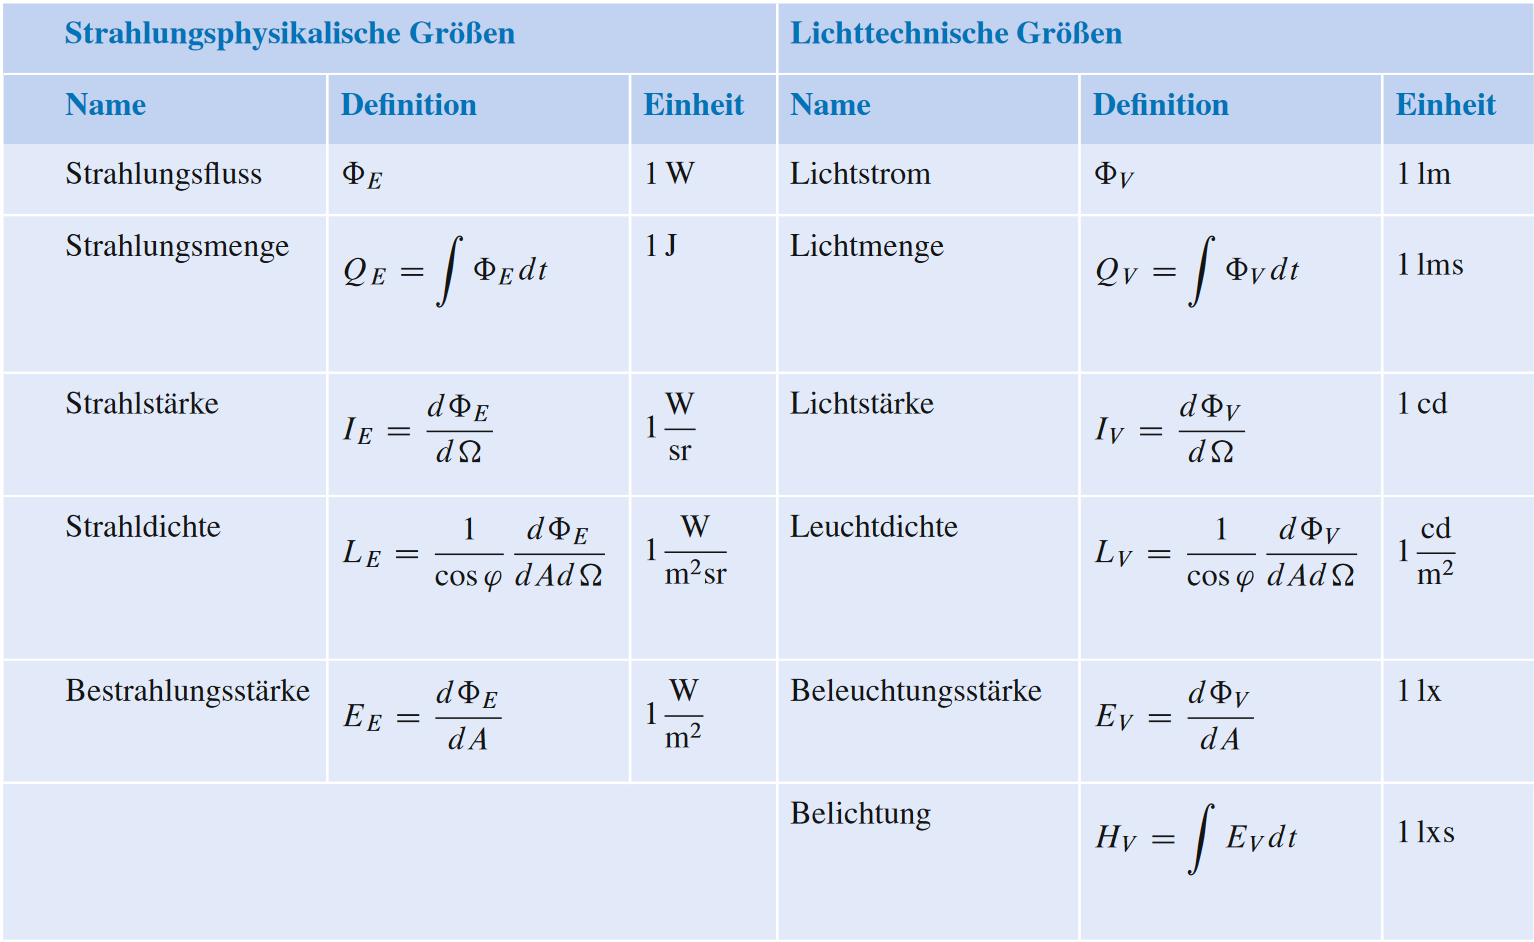
\includegraphics[width=.5\textwidth]{1.png}
\end{figure}

\subsection{Gesetze}
\subsubsection{Stefan-Boltzmann-Gesetz:}\tight
    \begin{align*}
        \Phi_E &= \sigma \cdot A \cdot T^4\\
        \sigma &= 5.670 \cdot10^{-8} \ufrac{W}{m^2K^4}\note[Stefan-Boltzmann-Konstante]
    \end{align*}

\subsubsection{Wien'sches Verschiebungsgesetz:}
    Ist \(\lambda_{\te{max}}\) die Wellenlänge, bei der die Emission eines Schwarzerkörpers
    die maximale Intensität zeigt, so gilt:
    \begin{align*}
        \lambda_{max}\cdot T = \const = 2.8978 \E{-3} \mathrm{m\, K}
    \end{align*}

\subsubsection{Rayleigh-Jean-Gesetz:}
    Das Rayleigh-Jean-Gesetz beschreibt die Abstrahlungsleistungspektrum bei hohen Wellenlängen:
    \begin{align*}
        M_E(\lambda):= \frac{\mathrm  d \Phi_E(\lambda)}{\mathrm d\lambda}=2\pi k c\frac T{\lambda^4}
    \end{align*}

\subsubsection{Wien'sches Strahlungsgesetz:}
    Das Wien-Gesetz beschreibt die Abstrahlungsleistungspektrum bei niedrigen Wellenlängen:
    \begin{align*}
        M_E(\lambda) &= \frac{c_1}{\lambda^5} \frac{1}{e^{\frac{c_2}{\lambda T}}}
        = \frac{2\pi h  c^2}{\lambda^5} \frac{1}{e^{\frac{h c}{k_B}\frac{1}{\lambda T}}}
    \end{align*}

\section{Wellenoptik}
\subsection{EM-Wellen:}
Eine ebene Welle wird mathematisch beschrieben durch:
\begin{align*}
    \mat E = E_{0x} \e_x  e^{i(\omega t - kz)} + E_{0y} \e_y  e^{i(\omega t - kz + \delta)}
\end{align*}
Für \(\delta = 0\) ist die Welle linear polarisiert. Für 
\(\delta = \pm \frac \pi 2\) ist sie rechts-/linksdrehend.

Überlagern sich die Amplituden zweier kohärenter Wellen, so ist die 
Intensität:
\begin{align*}
    \braket I &= 4 \braket{I_0} \cos^2 \hug{\frac{\Delta \phi}{2}}
\end{align*}
 
Und allgemein für zwei Wellen mit Phasendifferenz \(\Delta\phi\):
\begin{align*}
    \braket{I} &= \varepsilon_0 c \braket[\big]{(\v E_1 + \v E_2)^2}\\
    &= \varepsilon_0 c \bug{\braket[\big]{\v E_1^2} + 2\braket[\big]{\v E_1 \v E_2} + \braket[\big]{\v E_12^2}}\\
    &= \braket[\big]{I_1} + \braket[\big]{I_{12}} + \braket[\big]{I_2}\\
    \braket{I_{12}} &= \varepsilon_0 c E_{01} E_{02} \cos(\Delta \phi)
    = \varepsilon_0 c \sqrt{\braket{I_1}\braket{I_2}} \cos(\Delta \phi)
\end{align*}

\subsection{Kohärenz}
\subsubsection*{Zeitliche Kohärenz}
Zeitspanne \(\Delta t_c\) in der sich die Phasendifferenz 
\(\Delta\phi_{12}(\v r, t) = \phi_1(\v r, t) - \phi _2(\v r, t)\) um weniger als
\(2\pi\) ändert. 

Man definiert hier auch die Kohärenzlänge \(\Delta l_c= c\cdot \Delta t_c\).

\subsubsection*{Räumliche Kohärenz}
Analog definiert man die räumlihe Kohärenz, wenn eine Wellenfront ihre Phasendifferenz
\(\Delta\phi_{12}(\v r, t) = \phi_1(\v r, t) - \phi _2(\v r, t)\) zwischen zwei 
an zwei Orten um weniger als \(2\pi\) ändert.

\subsubsection*{Kohärenzlänge realer Lichtquellen}
Die Emission eine Wellenzuges durch ein angeregtes Atom dauert ca. 1 bis 10ns 
(\(=\Delta t_c\)). In einem Wellenzug koexistieren verschiedene Frequenzen, die einer 
Verteilung folgen. Man nennt \(\Delta f = \frac 1{\Delta t_c}\) die Frequenzbreite.
Die Kohärenzlänge lasst sich in erster Näherung berechnen als 
\(l_c = \frac{\lambda^2}{\Delta \lambda}\).

\subsection{Interferenzphänomene}
\subsubsection{Doppenspalt:}\tight
\begin{align*}
    &\te{Maxima:} & \sin\theta_{max} &= \frac{n\lambda}{d}\\    
    &\te{Minima:} & \sin\theta_{min} &= \hug{n+\frac12}\frac{\lambda}{d}  
\end{align*}

\subsubsection{Einzelspalt:}\tight
\begin{align*}
    &\te{Maxima:} & \sin\theta_{max} &=  \hug{n+\frac12}\frac{\lambda}{d}\\    
    &\te{Minima:} & \sin\theta_{min} &= \frac{n\lambda}{d}    
\end{align*}

\subsubsection{Gitter:}\tight
\begin{align*}
    &\te{Maxima:} & \sin\theta_{max} &=  \frac{n\lambda}{d}\\    
    &\te{Minima:} & \sin\theta_{min} &= \frac{n\lambda}{d}    
\end{align*}

\subsubsection{Lochblende:}\tight
\begin{align*}
    &\te{Minimum:} & \sin\theta_{min} &=  1.22\frac{\lambda}{D}
\end{align*}

\subsection{Beugungsphänomene}
\subsubsection*{Frauenhofer Beugung:}
Abstand des Objektes zum Schirm  gro{\ss} \(\to\) Stahlen annähernd parallel
\(\to\) Beugungsbild nur Richtungsabhängig.

\subsubsection{Fresnel Beugung:}
Abstand des Objektes zum Schirm \emph{nicht} gro{\ss} \(\to\) 
Stahlen nicht parallel \(\to\) Beugungsbild Distanz und Richtungsabhängig.

\subsubsection{Fresnel-Kirchhoff'sches Beugungsintegral}
Die Amplitude und Phase auf einem Schirm \((z=0)\) sei durch \(\vec E_0(x,y)\) 
und \(\phi(x,y)\) gegeben. Dann ist die Amplitude an einem
Punkt $P=(x,y,z)^T$:
\begin{align*}
    \vec E_P(x,y,z) &= \iint\limits_{z=0} K(\beta)\frac{\vec E_0(x',y')}{r_A} 
    e^{i(\phi(x',y') - k r_A)} \dx'\dy'\\
    \te{mit } r_A &= \sqrt{(x-x')^2 + (y-y')^2 + z^2}
\end{align*}

\subsubsection{Fresnel-Linse}\tight
\begin{align*}
        &\te{Radien:}  & r_n &= 
        \sqrt{n\lambda f + \frac{n^2\lambda^2}4} \overset{f\gg n\lambda}{\approx} \sqrt{n\lambda f}
\end{align*}

\subsubsection{Lochblende}
Position der ersten Minima und Maxima hinter einer Lochblende. 
Angegeben sind die Werte für $\frac{k D}{2\pi} \sin \theta_{min}$ bzw. 
$\frac{k D}{2\pi} \sin \theta_{max}$. 
Au{\ss}erdem ist die Intensität der Nebenmaxima im Verhältnis zum zentralen
Maximum angegeben.
\begin{figure}[H]
    \centering
    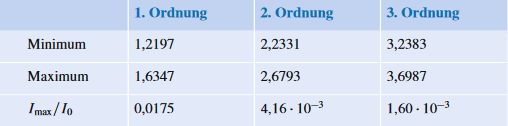
\includegraphics[width=0.5\textwidth]{2.png}
\end{figure}

\subsubsection{Rayleigh-Kriterium}
Die maximale Auflösung eines optischen Systems ist durch Beugungseffekte am 
Rand der Linse fundamental beschränkt. 
Das Rayleigh-Kriterium definiert die minimale auflösbare Winkeldistanz
als die Winkeldistanz bei der 
sich das Beugungsminimum erster Ordnung, des einen Objektes, mit dem
Beugungsmaximum erster Ordnung, des anderen Objektes, überlappen würde:
\begin{align*}
    \sin\theta_{min} =  1.22 \frac{\lambda}{D}
    \ \ \implies \ \ r_{min} =  1.22 \frac{f \lambda}{D}
\end{align*}

\section{Polarisation}
\subsubsection{Allgemein}
\begin{enumerate}
    \item Lineare Polarisation:\\
    Ein Strahl, dessen \(\vec E\)-Feld in nur einer konstanten Ebene schwingt, z.B 
    $\vec E(\vec r) = \hat E e^{i(\vec k \vec r + \omega t)}$. Er kann als Superposition zweier zirkular polarisierter Strahlen dargestellt werden, 
    die konträren Drehsinn haben, z.B. überlagern sich die beiden Wellen $(x, )$.
    \item Zirkulare Polarisation:\\
    Ein Strahl, dessen \(\vec E\)-Feld im Betrag konstant ist, und um die Ausbreitungsrichtung
    kreist. Er kann als Überlagerung zweier orthogonaler, linear polarisierter
    Strahlen dargestellt werden, die zueinnander um \(90^\circ\) phasenverschoben sind,
    z.B. \((x, \sin x, \sin(x+\pi/2))\)
    \item Optische Achse (Kristalloptik):\\
    Die optische Achse ist bei einem anisotropen Kristall jene Achse, entlang derer 
    jede Polarisationsrichtung den gleichen Brechungsindex hat.
    \item Haubtschnitt:\\
    Der Haubtschnitt ist jene Ebene, die durch die optische Achse und die Ausbreitungsrichtung 
    des Lichts aufgespannt wird.
    \item (Au{\ss}er)Ordentlicher Strahl:\\
    Der ordentliche Strahl eines Lichtstrahls ist jeder Teil dessen \(\vec E\)-Feld \emph{senkrecht}
    zum Haubtschnitt schwingt. Beim au{\ss}erordentlichen findet die Schwingung dem entsprechend 
    in der Ebene (Haubtschnitt) statt.\\
    Die Brechungsindizes von ordentlichem und au{\ss}erordentlichem Strahl sind 
    jeweils \(n_o\) und \(n_{ao}\).
\end{enumerate}

\subsubsection{Polarisationsfilter (Gesetz von Malus)}
\begin{align*}
    I' &= I \cdot \cos^2(\Delta \theta)
\end{align*}

\subsubsection{Lambda/4-Plättchen}
\begin{align*}
\Delta \phi &=\frac{2\pi}{\lambda} d \,\Delta n
\end{align*}

\subsubsection{Fresnel'sche Formeln}
Trifft ein Lichtstrahl unter einem Winkel \(\alpha\) zum Lot auf eine Grenzfläche 
zweier Medien mit Brechungszahlen $n_1$ und $n_2$, so wird er in
einen reflektierten und einen gebrochenen Strahl aufgespalten. Ihre
Amplituden sind durch die Reflexions- und Transmissionskoeffizienten 
für die Anteile an Polarisation in der Einfallsebene (Index p) und
senkrecht dazu (Index n) gegeben:
\begin{align*}
    r_n &= \frac{n_1\cos\alpha - n_2\cos\beta}{n_1\cos\alpha + n_2\cos\beta}\\
    r_p &= \frac{n_2\cos\alpha - n_1\cos\beta}{n_2\cos\alpha + n_1\cos\beta}\\
    t_n &= \frac{2 n_1 \cos\alpha}{n_1\cos\alpha + n_2\cos\beta}\\
    t_p &= \frac{2 n_2 \cos\alpha}{n_2\cos\alpha + n_1\cos\beta}\\
\end{align*}

\subsubsection{Anisotropie durch Spannung}
Setzt man ein Material unter Spannung (Kraftvektor \(\v F\)), kann das Material 
anisotrop werden. Der ordentliche Strahl ist orthogonal zu \(\v F\), der
außerordentliche parallel.

\subsubsection{Faraway Effekt}
Linear polarisiertes Licht wird reist durch ein Material, das von einerm starken 
B-Feld entlang der Ausbreitungsrichtung durchsetzt ist. Es wird dabei 
um einen Winkel \(\alpha = V\, L \, B, \ V=\te{Verdet-Konstante}\) gedreht. Es lässt sich erklären, wenn man das linear polarisierte Licht als 
Überlagerung zweier zirkular polarisierter Strahlen betrachtet. 
Die beiden Wellen regen Elektronen zu einer Kreisbahn an, die einen Dipolmoment erzeugt,
der je nach Richtung energetisch günstig oder ungünstig im B-Feld liegt.

\subsubsection{Kerr-Effekt}
Equivalent zum Faraway Effekt, jedoch wird hier ein E-Feld angelegt. Es bildet sich erneut
ein anisotropes Material, da das äußere E-Feld die Schwingungseigenschaften der Elektronen 
beeinflusst. Die optische Achse liegt entlang der E-Feld Richtung.
Die Erzeugung von Dipolen ist proportional zu \(E\), und die Ausrichtung der 
Dipole auch, insgesamt also \(\propto E^2\):
\begin{align*}
    \Delta n &= n_{ao} - n_o = K \lambda E^2\note K=\te{Kerr-Konstante}\\
    \Delta \phi &= 2\pi L K E^2
\end{align*}

\subsubsection{Pockels-Effekt}
Wie Kerr-Effekt, jedoch linear in \(E\). Der Effekt ist um mindestens eine 
Größenordnung stärker als der Kerr-Effekt, bei gleicher Feldstärke.
Der Effekt ist stark Richtungsabhängig.
\begin{align*}
    \Delta n &= n_{ao} - n_o = n^3 r_{\te{eff}} E 
    \note r_{\te{eff}} = \te{effektiver elektrootischer Tensor}\\
\end{align*}

\subsubsection{Spiegel-Isomerie}
Eine Lösung mit chiralen Molekülen dreht den Winkel des einfallenden linear polarisierten
Licht. 
\begin{align*}
    \alpha &= [\alpha]^T_\lambda \cdot \beta \cdot L \\
    [\alpha]^T_\lambda &= \te{spezifischer Drehwinkekl}\\
    \beta &= \te{Konzentration}\\ 
\end{align*}

\section{Quantenphysik}
\subsection{De-Broglie-Wellenlänge}
\begin{align*}
    \v p &= \hbar \cdot \v k \rightarrow
    p = \hbar \cdot k = \frac{h c}{\lambda}
\end{align*}



\end{document}